\begin{frame}
	\begin{center}
		\Huge Daniel Jadanec
	\end{center}
\end{frame}

\begin{frame}
	 \begin{enumerate}
		 \item Mein Aufgabenbereich
		 \item Bisheriger Stand
		 \item Anforderung
		 \item Umsetzung
		 \item Ergebnis
		 \item Fazit
	\end{enumerate}
\end{frame}

\begin{frame}{Mein Aufgabenbereich}
	\begin{itemize}
		\item VR Trajectory Datei mit den Berechnungen von Vadere
		\item Bugfixes und Optimierung
		\item Bimodales Simulationsmodell
	\end{itemize}

	\begin{minipage}{0.4\textwidth}
		\begin{figure}
			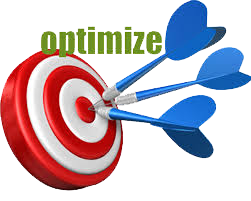
\includegraphics[width=\textwidth]{appendix/images/caricature/optimize.png}
		\end{figure}
	\end{minipage} \hfill
	\begin{minipage}{0.5\textwidth}
			\begin{figure}[H]
				
\includegraphics[width=\textwidth]{appendix/images/caricature/bugfixer.png}
			\end{figure}
	\end{minipage}
\end{frame}

\begin{frame}{Bisheriger Stand}
	\begin{itemize}
		\item Trajectory hatte keine Information über Agententypen
		\item Die Simulation lief nur mit einem Bewegungsmodell \cite{zarnitz-2015}
	\end{itemize}
\end{frame}

\begin{frame}{Anforderung}
	\begin{enumerate}
		\item VR Gruppe soll eine eigene Trajectory Datei bekommen
		\item Der Code soll für den letzten Sprint optimiert werden
		\item Mehrere Bewegungsmodelle sollen interagieren
	\end{enumerate}
\end{frame}

\begin{frame}{Umsetzung: UML Trajectory für VR}
	\begin{figure}
		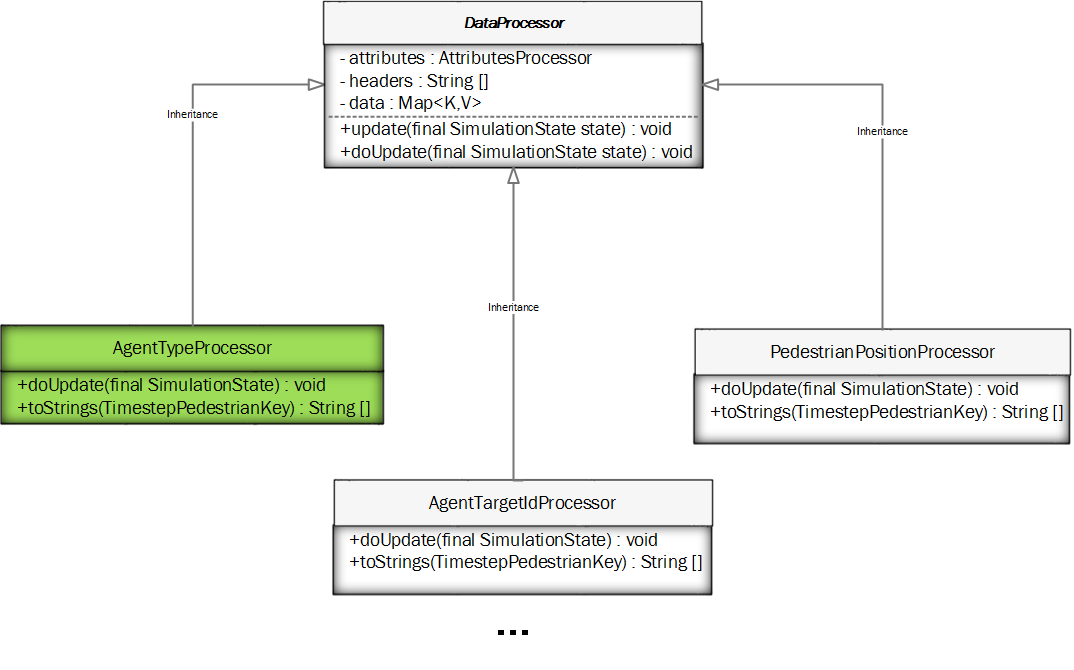
\includegraphics[width=\textwidth, keepaspectratio]{appendix/uml/OutputProcessor.png}
	\end{figure}
\end{frame}

\begin{frame}{Ergebnis: Trajectory für VR}
	\begin{minipage}{0.4\textwidth}
		\begin{itemize}
			\item Agent-Typ numerisch angegeben
			\item Leichte Ergänzung weiterer Prozessoren
			\item Datei exklusiv für die VR Gruppe und ihre Bedürfnisse angepasst
		\end{itemize}
	\end{minipage} \hfill
	\begin{minipage}{0.5\textwidth}
			\begin{figure}[H]
				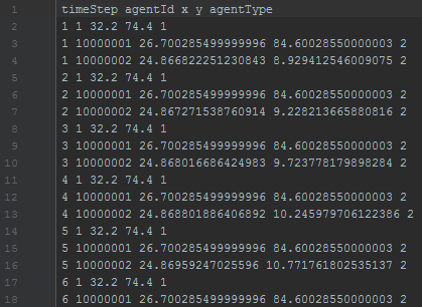
\includegraphics[width=\textwidth]{appendix/images/Trajectory.png}
			\end{figure}
	\end{minipage}
\end{frame}

\begin{frame}{Umsetzung: Bimodales Modell}
	\begin{figure}
		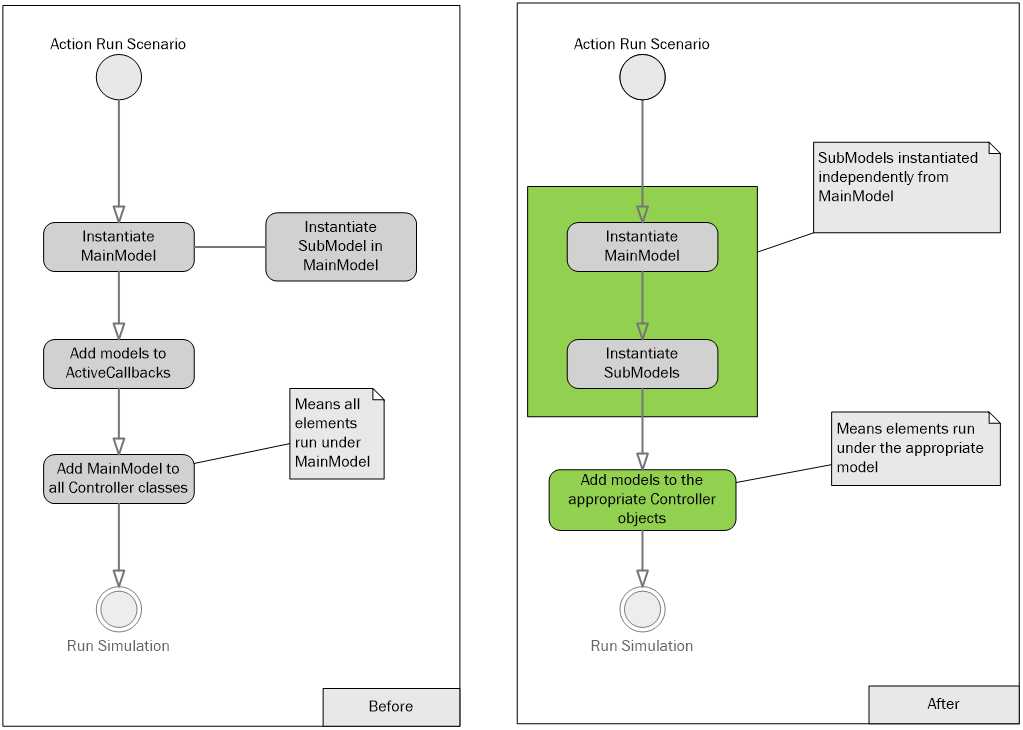
\includegraphics[width=\textwidth, height=0.8\textwidth, keepaspectratio]{appendix/uml/MotionModels.png}
	\end{figure}
\end{frame}

\begin{frame}{Änderung der Json Konfiguration}
	\begin{figure}
		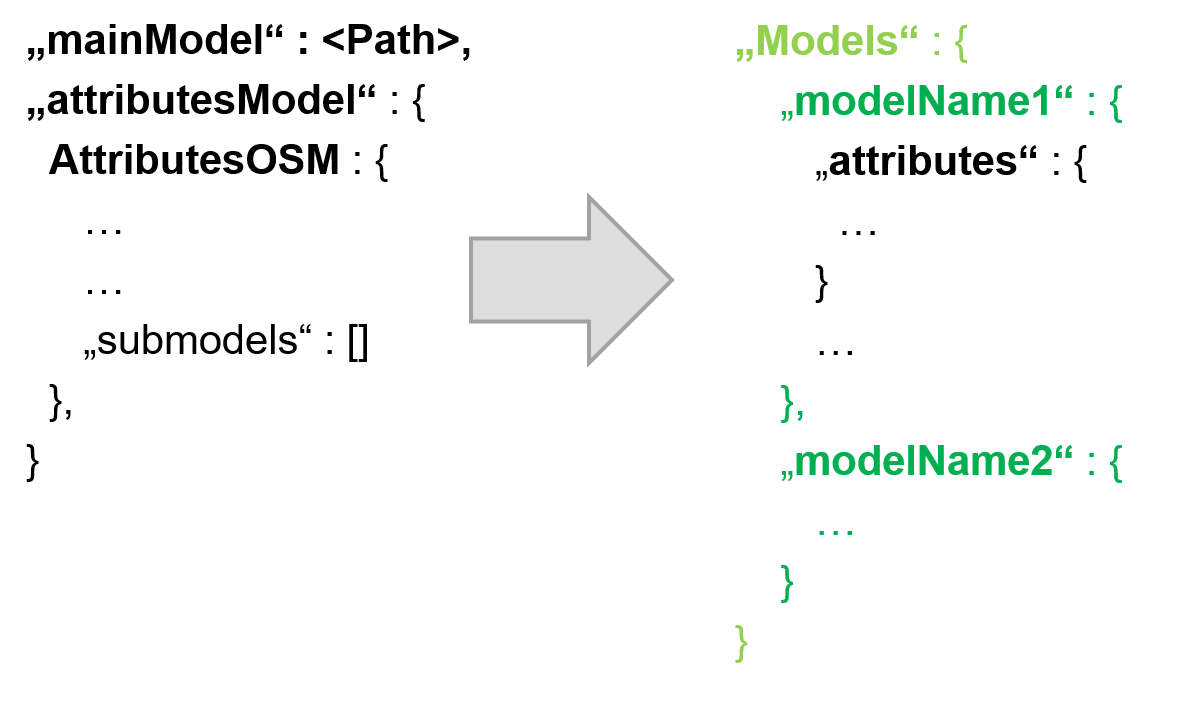
\includegraphics[width=\textwidth, height=0.8\textwidth, keepaspectratio]{appendix/images/JsonChange.png}
	\end{figure}
\end{frame}

\begin{frame}{Zweck der Änderung}
	\begin{itemize}
		\item	Mehrere Bewegungsmodelle erhalten nun Konfigurationsdaten
		\item Festlegen der Szenario Elemente, die mit dem Modell laufen sollen
		\item Der SubModel Knoten kann weitergeführt werden, nun aber als tatsächliches Untermodell
	\end{itemize}
\end{frame}

\begin{frame}{Ergebnis: Bimodales Modell}
	\begin{figure}
		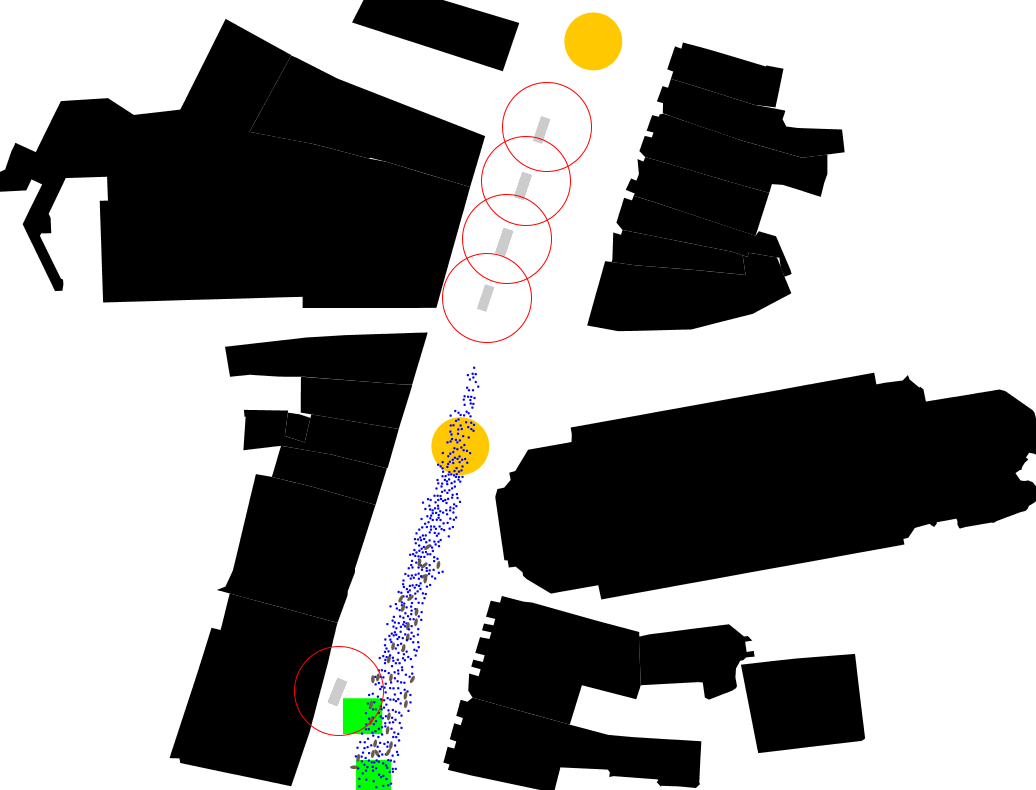
\includegraphics[width=\textwidth, height=0.7\textwidth, keepaspectratio]{appendix/images/landshutbimodal.png}
	\end{figure}
\end{frame}

\begin{frame}{Fazit}
	\par{Positiv:}
	\begin{itemize}
		\item Aufgabenzuweisung und Taskerstellung ging sehr schnell
		\item Scrum Master hielt das „Böse“ von uns fern
		\item Gut strukturierter Sprint mit festgelegten Meetings
	\end{itemize}

	\par{Ausbaufähig:}
	\begin{itemize}
		\item Gewicht/Schwierigkeit eines Tasks
		\item Mehr Tests sollten geschrieben werden
		\item Engere Zusammenarbeit mit den anderen Teams. Für den letzten Sprint unumgänglich!
	\end{itemize}

	\par{ Selbsteinschätzung: 23 \% }
\end{frame}
